\item \points{15} {\bf Logistic Regression: Training stability}

In this problem, we will be delving deeper into the workings of logistic
regression. The goal of this problem is to help you develop your skills
debugging machine learning algorithms (which can be very different from
debugging software in general).

We have provided an implementation of logistic regression in
\texttt{src/stability/stability.py}, and two labeled datasets $A$ and $B$ in
\texttt{src/stability/ds1\_a.csv} and \texttt{src/stability/ds1\_b.csv}.

Please do not modify the code for the logistic regression training algorithm
for this problem. First, run the given logistic regression code to train two
different models on $A$ and $B$. You can run the code by simply executing
\texttt{python stability.py} in the \texttt{src/stability} directory.

\begin{enumerate}

  \item \subquestionpoints{2}
What is the most notable difference in training the logistic regression model
on datasets $A$ and $B$?


\ifnum\solutions=1 {
  \begin{answer}

When running the logistic regression model on both datasets A and B, we notice that dataset A converges quickly after a few iterations. Dataset B goes through an infinite amount of iterations before converging. It does not get to achieve convergence because logistic regression cannot find a local optima when classes have a linear separation.

\end{answer}

} \fi

  \item \subquestionpoints{5}
Investigate why the training procedure behaves unexpectedly on dataset $B$, but
not on $A$. Provide hard evidence (in the form of math, code, plots, etc.) to
corroborate your hypothesis for the misbehavior. Remember, you should address
why your explanation does \emph{not} apply to $A$.

\textbf{Hint}: The issue is not a numerical rounding or over/underflow error.


\ifnum\solutions=1 {
  \begin{answer}

\begin{figure}[here]
   \centering
   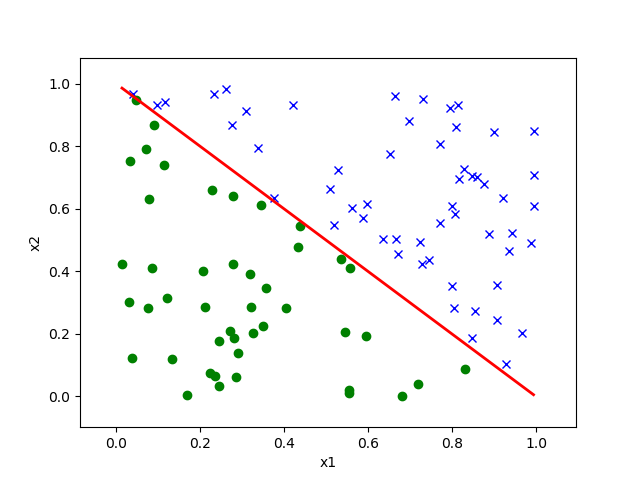
\includegraphics[width=4in]{fig_b.png} 
   \caption{Dataset B}
   \label{fig:separation}
\end{figure}

This figure plots Dataset B. We can see that the two classes [1,0] are well separated.
Separation occurs when variables are associated with only one outcome.
The problem is that when there is separation (the logistic curve lies strictly 0 or 1).
The optimization does not converge,  the model parameter goes to infinity when maximizing the likelihood of the function. The parameters continue increasing, as it tries to find an optimal separation of the classes. However, there is an infinite optimal values in which a linear boundary can form under well separated classes. 

\begin{figure} 
   \centering
   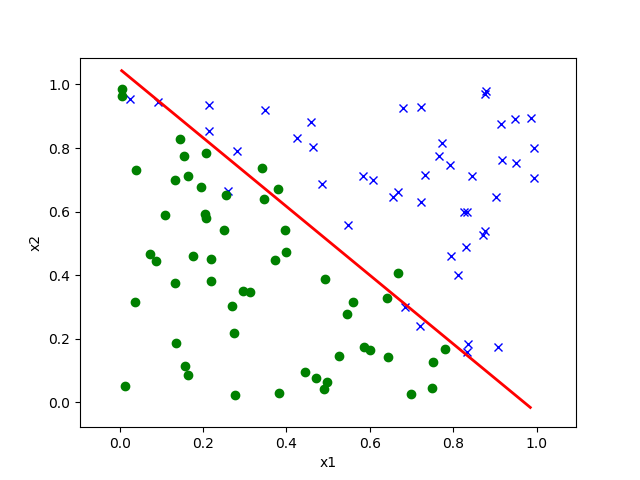
\includegraphics[width=4in]{fig_a.png} 
   \caption{Dataset A}
   \label{fig:separation}
\end{figure}

The Dataset A does not show complete separation of classes.

\end{figure}

} \fi


  \item \subquestionpoints{5}
For each of these possible modifications, state whether or not it would lead to
the provided training algorithm converging on datasets such as $B$. Justify your
answers.
\begin{enumerate}
  \item Using a different constant learning rate.
  \item Decreasing the learning rate over time (e.g. scaling the initial
  learning rate by $1/t^2$, where $t$ is the number of gradient descent
  iterations thus far).
  \item Linear scaling of the input features.
  \item Adding a regularization term $\|\theta\|_2^2$ to the loss function.
  \item Adding zero-mean Gaussian noise to the training data or labels.
\end{enumerate}
 


\ifnum\solutions=1 {
  \begin{answer}

i. No, different Learning rate: A constant learning rate will not help the coefficients converge. The constant learning rate will not prevent the parameters from continuing to increase to infinity. 

ii. No, decreasing the learning rate will usually cause the convergence to happen faster, however for dataset B, this won't help, as the classes are well separated, and reducing learning rate will not prevent the parameters from going to infinity values

iii. No, scaling the input features will not help in un-doing the separation of the classes. Scaling will transform the data, however, it will maintain similar proportions and the separation will still be present. Scaling the input features might even create more separation of the classes.

iv. Yes, adding regularization will help change the objective function changes with respect to the separation of the data. The objective will become "convex" even if the data is separated. The regularization will add penalty on the coefficient, and it will reduce the coefficient until it converges.

v.  Yes, adding zero mean gaussian noise might be able to help add data points to either class, and reduce the complete separation of the classes. The zero mean gaussian will only help if the noise added causes the data points for both classes to be more spread and not only belong to a single class.
\end{answer}

} \fi


  \item \subquestionpoints{2}
Support vector machines (SVMs) are an alternative machine learning model that we discussed in class.
We have provided you an SVM implementation (using a radial basis function (RBF) kernel) within \texttt{src/spam/svm.py} (You should not need to modify that code).

One important part of training an SVM parameterized by an RBF kernel (a.k.a Gaussian kernel) is choosing an appropriate kernel radius parameter.

Complete the \texttt{compute\_best\_svm\_radius} by writing code to compute the best SVM radius which maximizes accuracy on the validation dataset. Report the best kernel radius you obtained in the writeup.



\ifnum\solutions=1 {
  \begin{answer}
The best kernel radius that maximizes accuracy on the validation set is radius = 0.1.
It ended up showing an accuracy of 96.95 percent on the test set.

\end{answer}

} \fi

\end{enumerate}
